%!Mode:: "TeX:UTF-8"
\documentclass[a4paper,11pt,UTF8]{ctexart}

\usepackage{indentfirst} %缩进
\usepackage{xeCJK}    %使用系统字体
\usepackage{bm}       %粗体
\usepackage{fancyhdr} %自定义页眉页脚
\pagestyle{plain}                   %不设置页眉页脚
\usepackage{amsmath, amsthm, amssymb, amsfonts} %数学公式
\usepackage[a4paper,left=3cm,right=3cm,top=3.5cm,bottom=3.5cm]{geometry}
\usepackage{booktabs} %插入表格
\usepackage{diagbox}
\usepackage[section]{placeins} %避免浮动
\usepackage{listings} %插入代码
\usepackage{ctex}     %中文宏包
\usepackage[svgnames, table]{xcolor} %彩色表格
\usepackage{algorithm}          %伪代码
\usepackage{algorithmicx}
\usepackage{algpseudocode}
\usepackage{algorithm,algpseudocode,float}
\usepackage{lipsum}
\usepackage{enumitem}           %调整列举环境
\usepackage{url}
\usepackage{fontspec,xunicode}
\usepackage{subfigure}
\defaultfontfeatures{Mapping=tex-text} %如果没有它,会有一些 tex 特殊字符无法正常使用,比如连字符。

\usepackage{graphicx}
\graphicspath{{imgs/}}

%%%%%%%%%%%%%%%%%%%%%%%%%%%%%%%%%%%%%%%%%%%%%%%%%%%%%%%%%%%%%%%%
% 缩进及行间距
%%%%%%%%%%%%%%%%%%%%%%%%%%%%%%%%%%%%%%%%%%%%%%%%%%%%%%%%%%%%%%%%
\setlength{\parindent}{22bp} %重新定义缩进长度
\linespread{1}

%%%%%%%%%%%%%%%%%%%%%%%%%%%%%%%%%%%%%%%%%%%%%%%%%%%%%%%%%%%%%%%%
% 图的标题行间距设置
%%%%%%%%%%%%%%%%%%%%%%%%%%%%%%%%%%%%%%%%%%%%%%%%%%%%%%%%%%%%%%%%
\newcommand{\bottomcaption}{%
\setlength{\abovecaptionskip}{6bp}%
\setlength{\belowcaptionskip}{6bp}%
\caption}


%%%%%%%%%%%%%%%%%%%%%%%%%%%%%%%%%%%%%%%%%%%%%%%%%%%%%%%%%%%%%%%%
% 字体定义
%%%%%%%%%%%%%%%%%%%%%%%%%%%%%%%%%%%%%%%%%%%%%%%%%%%%%%%%%%%%%%%%
\setmainfont{Times New Roman}  %默认英文字体.serif是有衬线字体sans serif无衬线字体
\setmonofont{Consolas}
\setCJKmainfont[ItalicFont={楷体}, BoldFont={黑体}]{宋体}%衬线字体 缺省中文字体为
\setCJKsansfont{黑体}
\punctstyle{hangmobanjiao}
%-----------------------xeCJK下设置中文字体------------------------------%
\setCJKfamilyfont{song}{SimSun}                             %宋体 song
\newcommand{\song}{\CJKfamily{song}}
\setCJKfamilyfont{fs}{FangSong}                      %仿宋  fs
\newcommand{\fs}{\CJKfamily{fs}} 
\let\kaishu\relax                                    %重定义楷体,打开假粗体
\newCJKfontfamily\kaishu{KaiTi}[AutoFakeBold] 
%\setCJKfamilyfont{ktgb}{KaiTi_GB2312}                      %楷体 GB2312
%\newcommand{\ktgb}{\CJKfamily{ktgb}}
\setCJKfamilyfont{yh}{Microsoft YaHei}                    %微软雅黑 yh
\newcommand{\yh}{\CJKfamily{yh}}
\setCJKfamilyfont{hei}{SimHei}                              %黑体  hei
\newcommand{\hei}{\CJKfamily{hei}}
\setCJKfamilyfont{hwxk}{STXingkai}                                %华文行楷  hwxk
\newcommand{\hwxk}{\CJKfamily{hwxk}}
%------------------------------设置字体大小------------------------%
\newcommand{\chuhao}{\fontsize{42bp}{63bp}\selectfont}     %初号, 1.5倍行距
\newcommand{\xiaochuhao}{\fontsize{36bp}{36bp}\selectfont} %小初号,单倍行距
\newcommand{\yihao}{\fontsize{26bp}{39bp}\selectfont}        % 一号, 1.5 倍行距
\newcommand{\erhao}{\fontsize{22bp}{33bp}\selectfont}        % 二号, 1.5倍行距
\newcommand{\xiaoerhao}{\fontsize{18bp}{18bp}\selectfont}       % 小二, 单倍行距
\newcommand{\sanhao}{\fontsize{16bp}{24bp}\selectfont}       % 三号, 1.5倍行距
\newcommand{\xiaosanhao}{\fontsize{15bp}{22bp}\selectfont}      % 小三, 1.5倍行距
\newcommand{\sihao}{\fontsize{14bp}{21bp}\selectfont}        % 四号, 1.5 倍行距
\newcommand{\banxiaosi}{\fontsize{13bp}{20bp}\selectfont}  % 半小四, 20pt行距
\newcommand{\xiaosihao}{\fontsize{12bp}{20bp}\selectfont}       % 小四, 20pt行距
\newcommand{\dawuhao}{\fontsize{11bp}{11bp}\selectfont}      % 大五号, 单倍行距
\newcommand{\wuhao}{\fontsize{10.5bp}{10.5bp}\selectfont}   % 五号, 单倍行距
\newcommand{\xiaowuhao}{\fontsize{9bp}{9bp}\selectfont}   %小五号,单倍行距
%------------------------------重定义normalize------------------------%
\renewcommand{\normalsize}{\fontsize{12bp}{20bp}\selectfont}


%%%%%%%%%%%%%%%%%%%%%%%%%%%%%%%%%%%%%%%%%%%%%%%%%%%%%%%%%%%%%%%%
% 图题字体大小相同
%%%%%%%%%%%%%%%%%%%%%%%%%%%%%%%%%%%%%%%%%%%%%%%%%%%%%%%%%%%%%%%%
\usepackage{caption}
\captionsetup{font={footnotesize}}   % footnotesize = 9bp
\captionsetup[lstlisting]{font={footnotesize}}

%%%%%%%%%%%%%%%%%%%%%%%%%%%%%%%%%%%%%%%%%%%%%%%%%%%%%%%%%%%%%%%%
% 重定义枚举编号为 1),2)...
%%%%%%%%%%%%%%%%%%%%%%%%%%%%%%%%%%%%%%%%%%%%%%%%%%%%%%%%%%%%%%%%
\renewcommand{\labelenumi}{\theenumi)}


%%%%%%%%%%%%%%%%%%%%%%%%%%%%%%%%%%%%%%%%%%%%%%%%%%%%%%%%%%%%%%%%
% 重定义section标题
%%%%%%%%%%%%%%%%%%%%%%%%%%%%%%%%%%%%%%%%%%%%%%%%%%%%%%%%%%%%%%%%
\CTEXsetup[format={\CJKfamily{zhhei}\zihao{4}},number={\chinese{section}},name={,、~},aftername={},indent={0bp},beforeskip={6bp},afterskip={6bp},format+={\flushleft}]{section}
% \CTEXsetup[format={\Large\bfseries\CJKfamily{zhkai}\zihao{5}},name={(,)},number={\chinese{subsection}},aftername={},indent={22bp},beforeskip={6bp},afterskip={6bp}]{subsection}
\CTEXsetup[number={\chinese{section}},name={附录, ~~ }]{appendix}



%%%%%%%%%%%%%%%%%%%%%%%%%%%%%%%%%%%%%%%%%%%%%%%%%%%%%%%%%%%%%%%%
% 标题名称中文化
%%%%%%%%%%%%%%%%%%%%%%%%%%%%%%%%%%%%%%%%%%%%%%%%%%%%%%%%%%%%%%%%
\renewcommand\figurename{\hei 图}
\renewcommand\tablename{\hei 表}
\renewcommand\lstlistingname{\hei 代码}
\renewcommand{\algorithmicrequire}{\textbf{输入:}}
\renewcommand{\algorithmicensure}{\textbf{输出:}}
\newtheorem{define}{定义}


%%%%%%%%%%%%%%%%%%%%%%%%%%%%%%%%%%%%%%%%%%%%%%%%%%%%%%%%%%%%%%%%
% 列表设置
%%%%%%%%%%%%%%%%%%%%%%%%%%%%%%%%%%%%%%%%%%%%%%%%%%%%%%%%%%%%%%%%
\setlist[enumerate,1]{itemindent=22bp,listparindent=\parindent,itemsep=0mm,partopsep=.7mm,parsep=0ex,labelsep=1.5mm,topsep=0.7mm}
\setlist[enumerate,2]{label=\alph*),leftmargin=1.5em}  %二级item设置
%\setitemize{itemindent=38bp,leftmargin=0bp,itemsep=-0.4ex,listparindent=26bp,partopsep=0bp,parsep=0.5ex,topsep=-0.25ex}
%\setdescription{itemindent=38bp,leftmargin=0bp,itemsep=-0.4ex,listparindent=26bp,partopsep=0bp,parsep=0.5ex,topsep=-0.25ex}

%%%%%%%%%%%%%%%%%%%%%%%%%%%%%%%%%%%%%%%%%%%%%%%%%%%%%%%%%%%%%%%%
% 代码设置
%%%%%%%%%%%%%%%%%%%%%%%%%%%%%%%%%%%%%%%%%%%%%%%%%%%%%%%%%%%%%%%%
\lstset{
 columns=fixed,
 numbers=left,                                        % 在左侧显示行号
 numberstyle=\tiny\color{gray},                       % 设定行号格式
 frame=single,                                        % 单线背景边框
 breaklines=true,                                     % 设定LaTeX对过长的代码行进行自动换行
 keywordstyle=\color[RGB]{40,40,255},                 % 设定关键字颜色
 numberstyle=\footnotesize\color{darkgray},
 commentstyle=\it\color[RGB]{0,96,96},                % 设置代码注释的格式
 stringstyle=\rmfamily\slshape\color[RGB]{128,0,0},   % 设置字符串格式
 showstringspaces=false,                              % 不显示字符串中的空格
 language=java,                                        % 设置语言
 basicstyle=\linespread{1.0}\xiaowuhao\ttfamily,                      % 字体字号
 %lineskip=10bp,
 %baselinestretch=1,
}

%%%%%%%%%%%%%%%%%%%%%%%%%%%%%%%%%%%%%%%%%%%%%%%%%%%%%%%%%%%%%%%%
% 伪代码分页
%%%%%%%%%%%%%%%%%%%%%%%%%%%%%%%%%%%%%%%%%%%%%%%%%%%%%%%%%%%%%%%%
\makeatletter
\renewcommand{\ALG@name}{算法}
\newenvironment{breakablealgorithm}
  {% \begin{breakablealgorithm}
   \begin{center}
     \refstepcounter{algorithm}% New algorithm
     \hrule height.8bp depth0bp \kern2bp% \@fs@pre for \@fs@ruled
     \renewcommand{\caption}[2][\relax]{% Make a new \caption
       {\raggedright\textbf{\ALG@name~\thealgorithm} ##2\par}%
       \ifx\relax##1\relax % #1 is \relax
         \addcontentsline{loa}{algorithm}{\protect\numberline{\thealgorithm}##2}%
       \else % #1 is not \relax
         \addcontentsline{loa}{algorithm}{\protect\numberline{\thealgorithm}##1}%
       \fi
       \kern2bp\hrule\kern2bp
     }
  }{% \end{breakablealgorithm}
     \kern2bp\hrule\relax% \@fs@post for \@fs@ruled
   \end{center}
  }
\makeatother



\begin{document}
\xiaosihao\song

\begin{titlepage}
\center{\yihao{\hwxk{电子科技大学\underline{计算机科学与工程}学院}}}
\vspace{6cm}
\center{\xiaochuhao{\kaishu{\bfseries 实~验~报~告}}}
\vspace{4cm}

\begin{center}
\begin{large}
\begin{tabular}{rc}
\xiaoerhao{\hei{学\qquad 号}}& \hspace{1.7cm}\xiaoerhao{\hei{2020080903009\hspace{1.7cm}}} \\
\cline{2-2}\\
\xiaoerhao{\hei{姓\qquad 名}}& \xiaoerhao{\hei{李皓}}\\
\cline{2-2}\\
\xiaoerhao{\hei{(实验)课程名称}}& \xiaoerhao{\hei{CUDA并行程序设计实验}}\\
\cline{2-2}\\
\xiaoerhao{\hei{教师}}& \xiaoerhao{\hei{卢国明}}\\
\cline{2-2}\\

\end{tabular}
\end{large}
\end{center}
\vfill \hfill
\end{titlepage}
\clearpage

\centerline{\\[10bp]\erhao{\fs{电 ~子 ~科~ 技~ 大~ 学}}}

\centerline{\\[20bp]\yihao{\fs{实  ~~~~ 验  ~~~~ 报  ~~~~ 告}}}

\leftline{\\[10bp]\sihao{\hei{\hspace{1.5em} 学生姓名:李皓 \hfill 学号:2020080903009 \hfill 指导教师:卢国明 }}}

% \leftline{\\[10bp]\sihao{\hei{\hspace{1.5em} 实验地点:信软楼西XXX \hfill }}}

% \leftline{\\[10bp]\sihao{\hei{\hspace{1.5em} 实验时间:第X周周X(X-X节) \hfill }}}

\setlength{\parskip}{0bp}  %定义段间距

\section{实验名称: N-Body问题并行程序设计及性能优化}
% \section{实验学时: ~4}
\section{实验目的:}
\begin{enumerate}
  \item 实现N-body的cuda并行算法。
  \item 使用各种方法对程序进行调优。
\end{enumerate}

\section{实验原理:}

\subsection{N-Body问题概述}

N-body问题(或者说N体问题),是一个常见的物理模拟问题。在N-body系统中,每个粒子体都会与剩下的其他粒子产生交互作用(交互作用因具体问题而异),从而产生相应的物理现象。天体模拟就是一个非常经典的N-body系统,根据牛顿的万有引力定律,宇宙中的不同天体之间会产生相互作用的吸引力,吸引力根据两个天体之间的质量和距离的不同而各不相同,一个天体的运动轨迹最终取决于剩下的所有的天体对该天体的引力的合力。

\subsection{N-body问题的CUDA实现}

\begin{enumerate}
  \item 串行算法
  
  串行算法只使用了CPU串行计算粒子间引力并更新位置,还未引入CUDA使用GPU并行计算。
首先,对每个点的位置和速度进行随机初始化。
然后,根据位置进行计算相互的作用力,以此为依据更新点的速度。
根据新的速度,更新每个点的位置,然后开始下一个周期的计算。

  \item 并行算法
  
  由于在同一周期内计算每一个点的受力情况是相互独立互不影响的,可以利用GPU高达数千核的并行计算特点,用n个线程并发计算速度的变化,每个线程处理一个粒子的计算任务,然后再用n个线程并发更新位置。
在CUDA编程中,设备端指GPU端,数据存放在显存中;主机端指CPU,数据存放在内存中。一般情况下,设备端是不能直接访问主机端内存的,而数据通常情况下都是存放在主机端内存中,要在GPU中执行算法运算就必须先把数据拷贝至设备端,运算完成再把结果拷回至主机端。

\end{enumerate}

\section{实验内容:}

\begin{enumerate}
  \item 学习和使用集群及CUDA编译环境
  \item 基于CUDA实现N-Body 程序并行化
  \item N-Body并行程序的性能优化
  
\end{enumerate}

\section{实验设备:}

\begin{enumerate}
  \item 操作系统:Windows 11 专业版
  \item CPU: Ryzen 5-5700X
  \item 编程环境:vscode
  \item 执行环境:实验室服务器集群
  \item Node-CPU: Intel(R) Xeon(R) Gold 5318Y x2
  \item GPU: Nvidia K80*2
  \item 操作系统:CentOS 7.2
  \item CUDA:10.0
  \item 内存:64G
  
\end{enumerate}
\section{实验步骤}

下面进行实验操作:
\subsection{环境连接和配置}
为了在cuda机上进行开发,因此需要连接到相应的机器上进行在线配置和链接。首先配置ssh config文件:
\begin{lstlisting}
Host CUDA
  HostName mpi-cu08-1
  ProxyJump MPI
  User 2020080903009

Host MPI
  HostName 121.48.170.9
  User 2020080903009
  Port 10022
\end{lstlisting}

随后进行链接后可以直接打开远程工作区进行开发。如下图所示:
\begin {figure}[h]
\centering % 居中显示
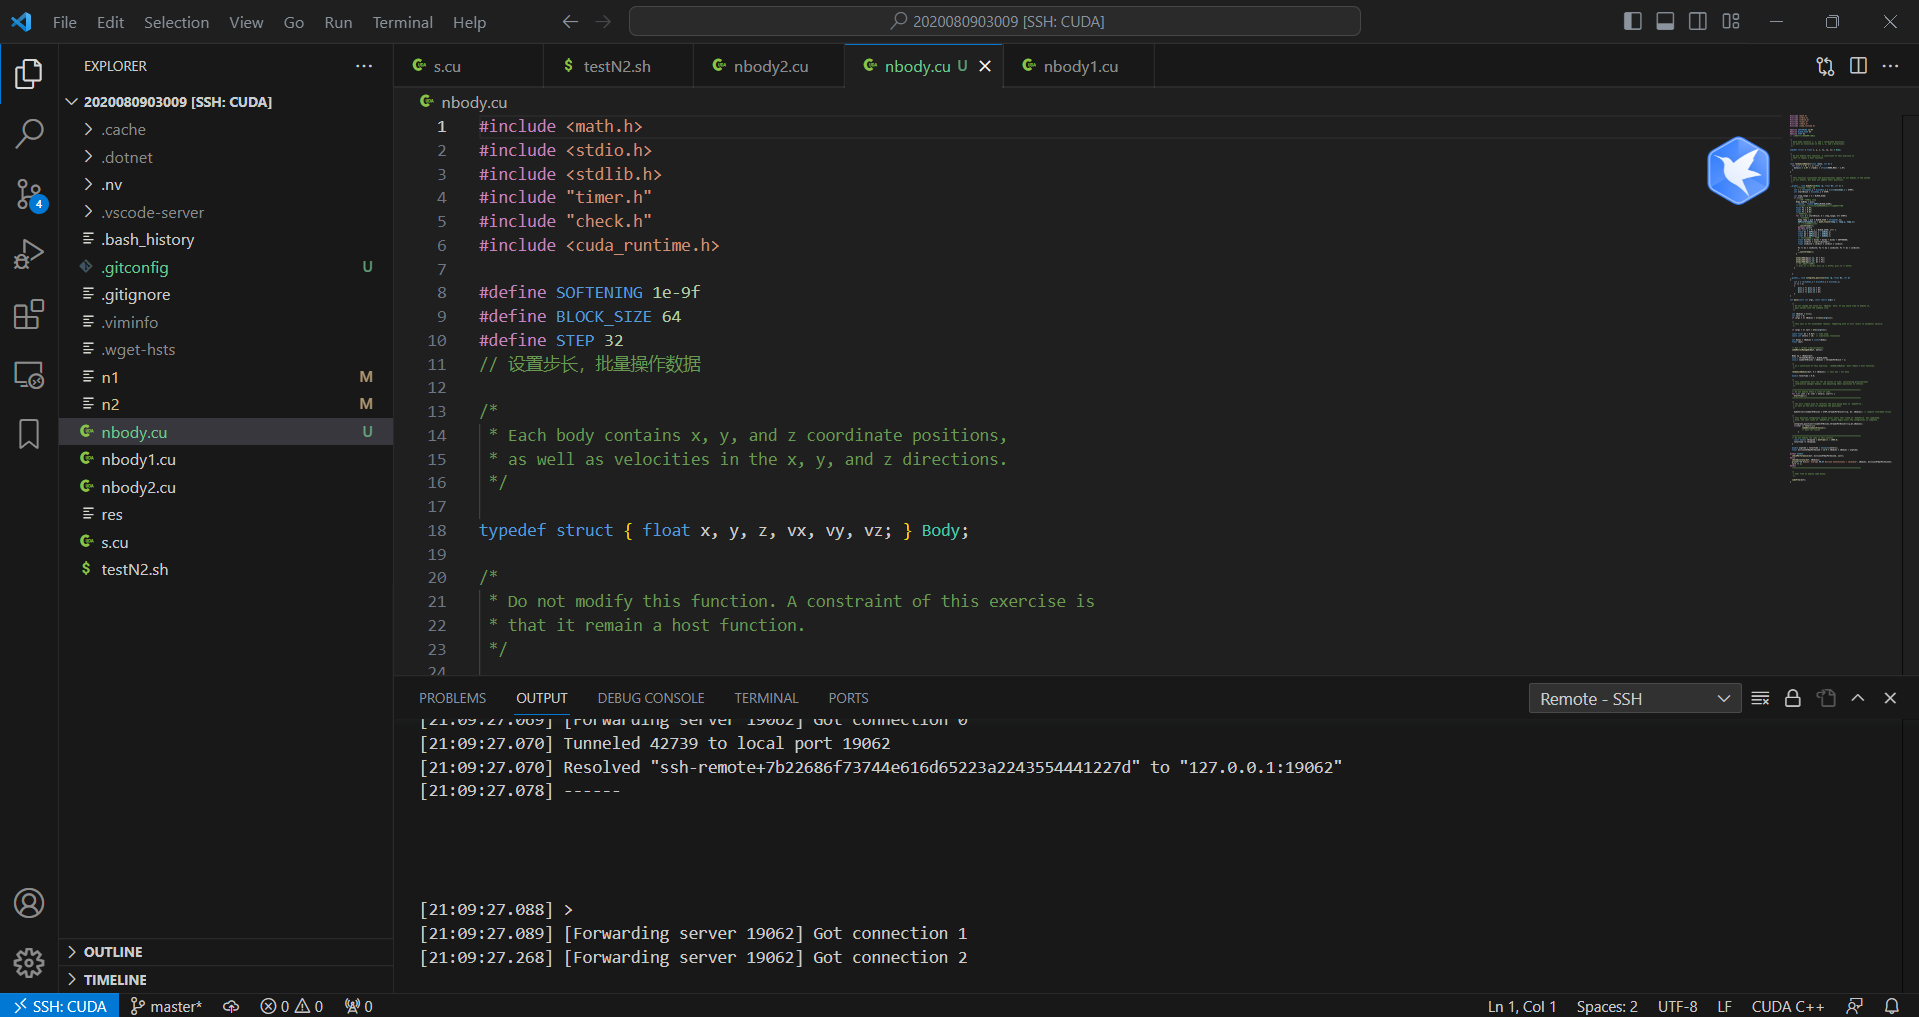
\includegraphics[width=\textwidth]{1602-051421.png}
\caption{远程开发示例} % 标题
\label{five}
\end {figure}
\newpage

利用基本的代码进行性能和环境测试。首先编译代码:
\begin{lstlisting}
  2020080903009@mpi-cu08-1: nvcc -arch sm_37 -o s s.cu
\end{lstlisting}
\begin {figure}[h]
\centering % 居中显示
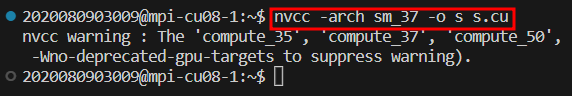
\includegraphics[width=\textwidth]{2204-051421.png}
\caption{代码编译运行结果} % 标题
\label{five}
\end {figure}

随后运行,测试代码运行的效果:

\begin {figure}[h]
\centering % 居中显示
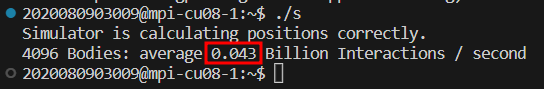
\includegraphics[width=\textwidth]{2501-051421.png}
\caption{基准代码测试结果} % 标题
\label{five}
\end {figure}

可见由于使用CPU来进行位置的模拟,只能做到有限的并行,因此程序在一定时间内作出的交互行为有限。接下来的目标就是利用GPU加速运行,使得程序加速。

\subsection{并行化操作}

在计算更新粒子位置的时候,需要根据粒子间的相对位置计算力的大小,得到各个方向的加速度vx,vy,vz,随后更新当前的位置信息。显然,计算加速度的过程中能够并行进行计算,这是因为计算位置的行为没有结果的依赖。只需知道当前粒子的位置和相对的位置,根据万有引力公式计算出该对粒子产生出来的加速度。

为了对此过程进行优化,需要将计算距离的函数 bodyForce 函数,integrate position 函数进行修改,使之成为在cuda设备上计算运行的函数。为了存储结果,还需要在显存中分配空间存储粒子的状态信息。如下是分配显存的部分代码:

\begin{lstlisting}[language=C++]
  int bytes = nBodies * sizeof(Body);
  float *buf;
  // buf = (float *)malloc(bytes);
  cudaMallocManaged(&buf, bytes);
  Body *p = (Body*)buf;
\end{lstlisting}

使用cudaMalloc命令完成分配,随后分析代码的并行方法。由于每次位置迭代是所有粒子(4096个)都参与运算,因此需要为每个粒子的位置迭代进行线程的分配。受限于显卡的并行架构设计,线程要以线程块的形式分批计算。随后规定进程块的大小和个数:

\begin{lstlisting}[language=C++]
  size_t threadsPerBlock = BLOCK_SIZE;
  size_t numberOfBlocks = nBodies / threadsPerBlock + 1;
\end{lstlisting}

随后进行设备代码的修改,对于bodyForce代码而言,需要先计算出自身进程所对应的索引,这个行为是由块号和块内ID所参与计算的。随后迭代计算即可,该函数和原函数的差异之处在于将外层的循环进行了优化,使得4096个粒子都在并行计算。在调用函数的过程则传入了块数量和每块线程的线程数。代码修改如下:
\begin{lstlisting}[language=C++]
// 调用函数
bodyForce<<<numberOfBlocks,threadsPerBlock>>>(p, dt, nBodies); // compute interbody forces
// 函数入口
__global__ void bodyForce(Body *p, float dt, int n) {
    int i = threadIdx.x + blockDim.x * blockIdx.x;
    // 取消了i的循环,计算每个进程对应的i
    float Fx = 0.0f;
    float Fy = 0.0f;
    float Fz = 0.0f;
    if (i<n){
      
      for (int j = 0; j < n; j++) {
        float dx = p[j].x - p[i].x;
        float dy = p[j].y - p[i].y;
        float dz = p[j].z - p[i].z;
        float distSqr = dx*dx + dy*dy + dz*dz + SOFTENING;
        float invDist = rsqrtf(distSqr);
        float invDist3 = invDist * invDist * invDist;
        Fx += dx * invDist3; Fy += dy * invDist3; Fz += dz * invDist3;
    }

    p[i].vx += dt*Fx; p[i].vy += dt*Fy; p[i].vz += dt*Fz;
    } 
  }
\end{lstlisting}

对于粒子的位置更新问题,由于加速度已经计算出来,因此直接计算更新后的位置即可。

\subsection{自由优化}

在完成基本的优化后,代码还有进行调整的空间。在计算各个粒子对之间产生的引力和加速度方面,还是使用了循环遍历所有的粒子。这部分可以进行并行化改进。可以通过分配更多的进程来完成计算,为此,引入变量STEP,每个STEP之间计算引力的行为可以并行操作。

引入STEP后对函数内的循环进行重构,使得每次循环都由原来的$n/BLOCK\_SIZE$次变为了$n/(BLOCK\_SIZE*STEP)$次。通过测试不同的STEP,可以有效加大代码的并行度,提高程序的执行效率。随着并行度的增加,对于加速度累计的情况,需要进行互斥相加的操作,使用函数atomicadd来实现。

该部分代码改动如下:
\begin{lstlisting}[language=C++]
  __global__ void bodyForce(Body *p, float dt, int n) {
    // 计算力的过程并行化
    int i = threadIdx.x + blockDim.x * (int)(blockIdx.x / STEP);
    int startBlock = blockIdx.x % STEP;
    
    int step_range = n / BLOCK_SIZE;
    if (i<n){
      // 设置标志记录 step
      Body myBody = p[i];
      __shared__ float3 bdPos[BLOCK_SIZE];
      // float3 是三个float构成的数据类型,共享以访问
      float Fx = 0.0f;
      float Fy = 0.0f;
      float Fz = 0.0f;
      // 批量间串行:
      for (int k = startBlock; k < step_range; k+= STEP){
        // 同步数据
        Body temp = p[k * BLOCK_SIZE + threadIdx.x];
        bdPos[threadIdx.x] = make_float3(temp.x, temp.y, temp.z);
        // 阻塞等待数据同步
        __syncthreads();
        #pragma unroll
        for (int j = 0; j < BLOCK_SIZE; j++) {
        float dx = bdPos[j].x - myBody.x;
        float dy = bdPos[j].y - myBody.y;
        float dz = bdPos[j].z - myBody.z;
        // 从自己的块进行访问
        float distSqr = dx*dx + dy*dy + dz*dz + SOFTENING;
        float invDist = rsqrtf(distSqr);
        float invDist3 = invDist * invDist * invDist;
        Fx += dx * invDist3; Fy += dy * invDist3; Fz += dz * invDist3;
        }     
        __syncthreads();
      }

      atomicAdd(&p[i].vx, dt * Fx);
      atomicAdd(&p[i].vy, dt * Fy);
      atomicAdd(&p[i].vz, dt * Fz);
      // 并行化防止脏操作
      // p[i].vx += dt*Fx; p[i].vy += dt*Fy; p[i].vz += dt*Fz;
    }
  }
\end{lstlisting}

\section{实验结果与分析:}
\subsection{并行化操作结果}
编译运行并行化的程序后,得到以下结果:
\begin {figure}[h]
\centering % 居中显示
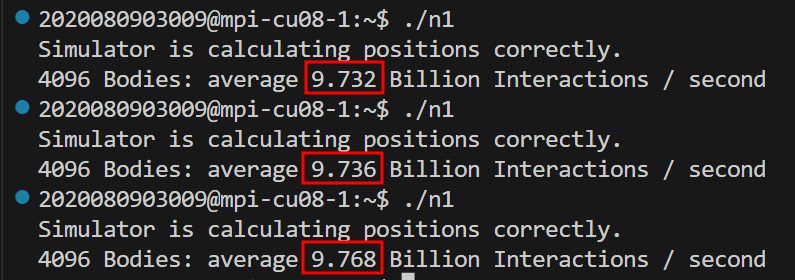
\includegraphics[width=\textwidth]{0311-051511.png}
\caption{并行化操作结果} % 标题
\label{five}
\end {figure}

和串行操作相比,每秒处理的运动迭代次数提升了227倍,没能够达到更高的提升倍数是因为并行操作的开销,以及函数内还有优化的空间。

\subsection{自由优化结果}

编译运行文件,得到以下结果:
\begin {figure}[h]
\centering % 居中显示
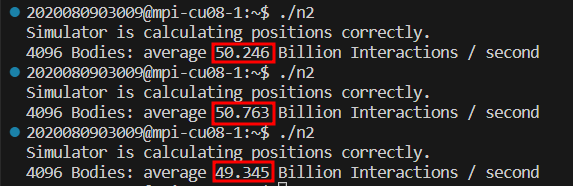
\includegraphics[width=\textwidth]{3112-051511.png}
\caption{自由优化后的运行结果} % 标题
\label{five}
\end {figure}

在之前的基础上通过分配更多的线程来完成并行计算的任务,速度提升了五倍。还使用了共享内存的方法来加速访问的效率,取得了较好效果。
\section{总结及心得体会:}

在本次实验中,我基本掌握了CUDA并行程序设计的方法。并且通过两次程序的优化,直观认识了不同性能优化方法的效果以及特点。

经过这次实验我对并行程序设计的优化有了新的认识,在后续的实践中可以对这些技巧灵活应用。

\section{对本实验过程及方法、手段的改进建议:}
在实验时需要对于CUDA的原理有更加深刻和直观的理解,需要在进行加强。

\vspace{4cm}
\begin{flushright}
\begin{tabular}{lc}
\sihao{\hei{报告评分:}}& \sihao{\vspace{10pt}}\\


\sihao{\hei{本人签字:}}&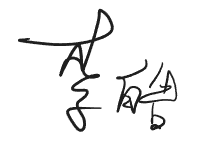
\includegraphics[width=60pt]{3341-041412.png}\\
\sihao{\hei{指导教师签字:}}& \sihao{\vspace{10pt}}\\

\end{tabular}
\end{flushright}

\newpage\section{代码清单}
\begin{enumerate}
  \item 代码I:CUDA并行
  
  \lstinputlisting[language=C++,linewidth=\textwidth]{o1.cpp}
  \item 代码II:优化
  
  \lstinputlisting[language=C++,linewidth=\textwidth]{o2}
\end{enumerate}

\end{document}
